\chapter{FacePush System} \label{chapter:system}
To render normal force feedback on the face, FacePush utilizes the original components of a Vive HMD\footnote{\url{https://www.vive.com/tw/}}, including face foam and belt. Just hereafter, we describe the hardware and software of our system as well as the mapping of motor rotations to apply pressure to the face.

\section{The Mechanical Design of FacePush OK}

\begin{figure}[h]
\begin{center}
    \begin{tabular}{@{\hspace{0.1cm}}c}
    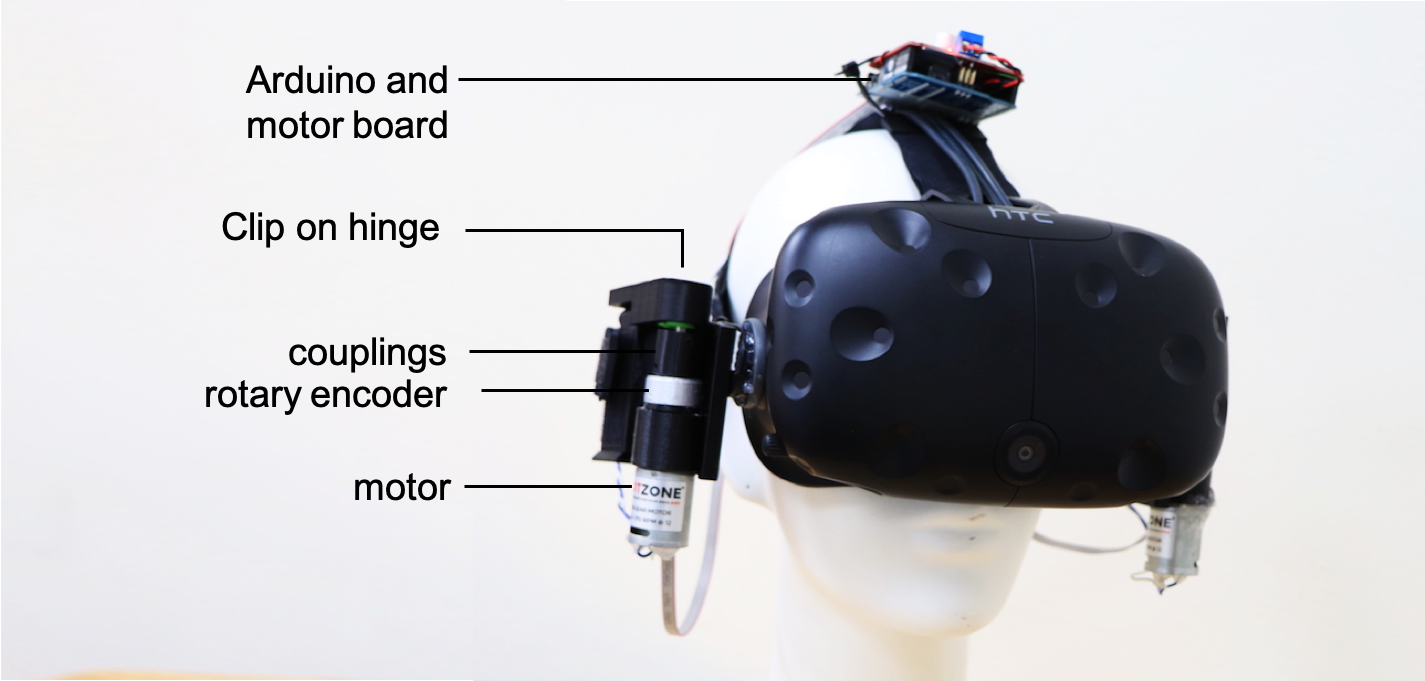
\includegraphics[width=1\textwidth]{figures/FrontView.png}
    \end{tabular}
    \caption{A front view of the FacePush system.}
    \label{fig:FrontView}
    \end{center}
\end{figure}

We considered the haptic feedback acting on the face as an embedded component installed in the HMD itself. The contact region of the foam in the HMD is a natural haptic space and the belt of the HMD, which is similar to a goggle strap,can provide  enough  constraint  to  tighten  the  headset. By tightening this belt, the user will experience a force like the face being pushed forward as pressure acts upon the face.

% In this case, 
We tested several different specifications of DC motors. Based on our experience and through design iterations, we suggest that the torque should exceed 2 N-m to provide enough power to pull the belt. However, their weight and size should be less than 100g, otherwise, the weight of the motor will restrict the movement of the user and reduce usability. We chose the 170 RPM Econ Metal Gearmotor, weighing at 92.1g, as the force actuators in our system. These motors are driven through an external motor driver (VNH2SP30-E) by a pulse width modulation (PWM) signal, with a power supply rated at 12V, 3.8A. In addition, the motors are controlled by a proportional-integral-derivative (PID) controller to ensure high positional accuracy. The PID loop iterates on an Arduino UNO board interfaced with a PC using a USB serial connection running at a 9600 baudrate.

\subsection{Torque Generators OK}

\begin{figure}[h]
\begin{center}
    \begin{tabular}{@{\hspace{0.1cm}}c}
        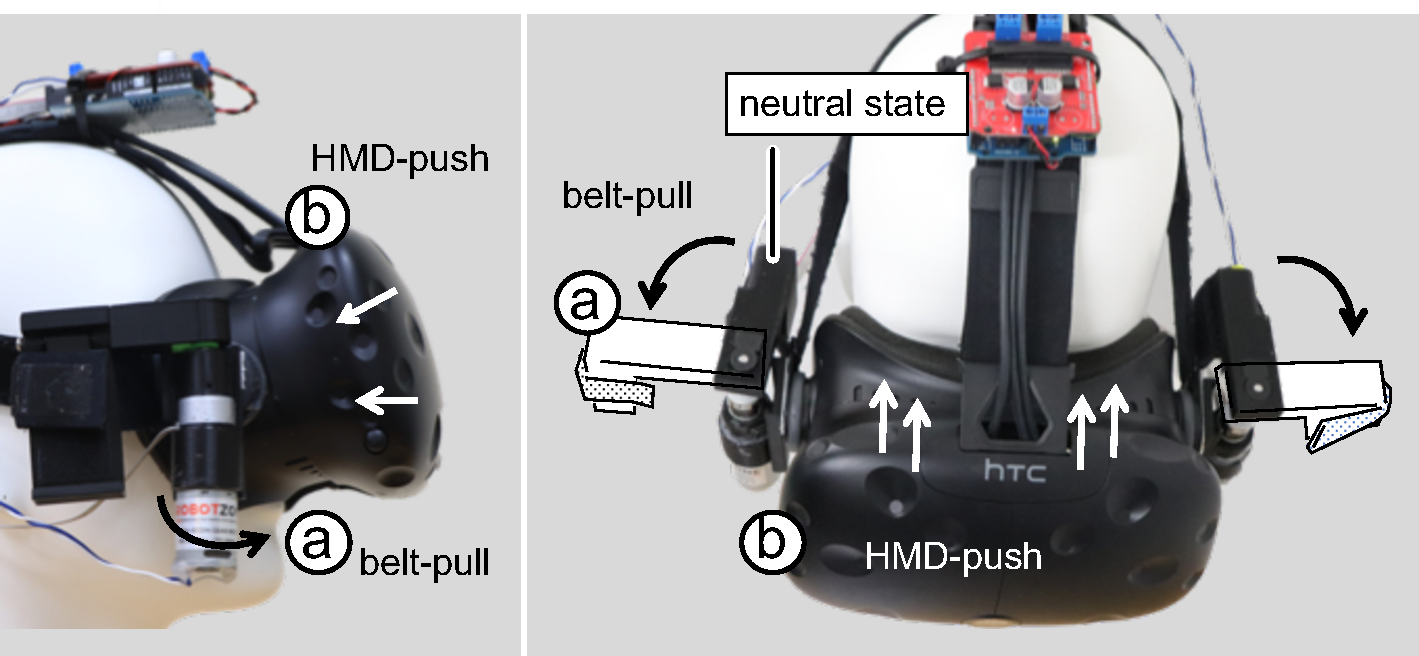
\includegraphics[width=1\linewidth]{figures/mechanical-design3}
    \end{tabular}
    \caption{Each motor connecting a belt via a torque generator allows (a) translate a belt-pull into (b) a HMD-push, resulting in a normal force on face.}
    \label{fig:mechanical_design}
 \end{center}
\end{figure}

As shown in Figure \ref{fig:FrontView}, two 3D-printed components are driven by the motors which were designed to fulfill these needs. These 3D-printed components, or torque generating components, are connected to the motor shaft through the coupling and they have a clip-on-hinge structure to grip the belt of the HMD and fasten them further when they are turned by the motor. (Hereafter these components will be referred to as ``torque generators'' for brevity.) Each motor has a rotary encoder attached to the shaft for recording its current position. The torque generators are attached to the left and right sides of the HMD. The clip structure and Velcro fasteners allow users to adjust the initial tautness of the belt (Figure \ref{fig:assemblyandsystem} a-c). 

\begin{figure}[hp]
\begin{center}
    \begin{tabular}{@{\hspace{0.1cm}}c}
    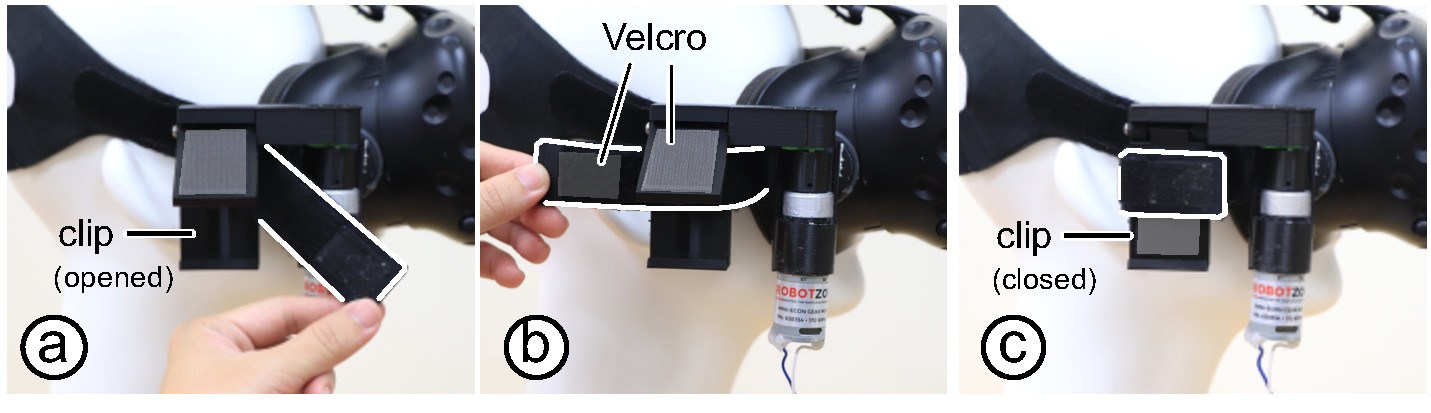
\includegraphics[width=1\textwidth]{figures/AssemblySystem.pdf}
    \end{tabular}
    \caption{(a)(b)(c) Assembly of FacePush on the HMD. The belt and the Velcro fasteners are touched for clarity.}
    \label{fig:assemblyandsystem}
    \end{center}
\end{figure}

Our torque generators transfer the torque generated by the motor shaft into a force exerted on the face. As displayed in Figure \ref{fig:mechanical_design}, we define the neutral state of FacePush as being when the torque generators are positioned parallel to the direction of a user facing forward. This is also the initial state of each ``push'' or application of force, so that each push has a reference point.

We assign the angle of the torque generators to 0 degrees. Both components can rotate at most 170 degrees, moving clockwise to the left and counterclockwise to the right. When the torque generators leave their neutral state, the belt is pulled tight and the user's face is forced forward. This force makes the entire HMD tighter and the user will experience a normal force acting on her/his face. 

\subsection{Two States of FacePush OK}

According to the position of the torque generators, we define two states for the behavior of FacePush. First one is \textit{Neutral State} (Figure \ref{fig:2_States} a). The neutral state represents torque generating components are positioned parallel to the direction of a user facing forward. At this moment, The rotate angle is 0 and there is no normal force exerted on the user's face. When the motor rotates, it drives the 3D-printed components and the belt is pulled. The belt-pull leads to a HMD-push resulting a normal force exerted on the user's face. We define this situation as \textit{Push State} (Figure \ref{fig:2_States} b). It represents the torque generating component is rotated and translates a belt-pull into a HMD push. At this moment, we can assign the angle to generate different magnitude of normal force during the Push State. Then, based on the behavior of the normal force, we design two different types of stimuli.

\begin{figure}[h]
\begin{center}
    \begin{tabular}{@{\hspace{0.1cm}}c}
    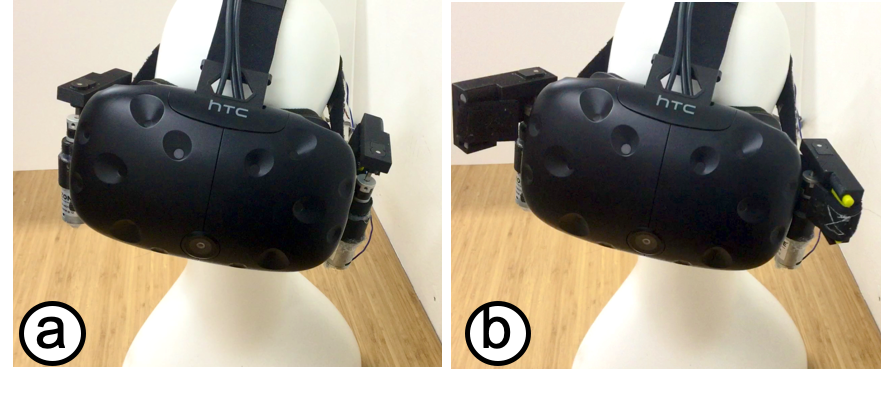
\includegraphics[width=1\textwidth]{figures/2_StatesOfFacePush.png}
    \end{tabular}
    \caption{(a)Neutral State: There is no normal force generated, when the rotate angle is 0.(b)Push State: Generates a variety of magnitude of normal force with different angle}
    \label{fig:2_States}
    \end{center}
\end{figure}

\subsection{\textcolor{red}{Two Types of Stimuli 文字 照片}}

\textcolor{red}{ 要再重新寫過 FacePush can generate either a weak, or a strong, stimulus based on the pressure intensity at different angles. We define two types of stimuli according to their implementation in our example applications. 1) Discrete stimulus: The duration is 0.5 seconds. Thus its impulse increases and decreases instantly; this is utilized in our boxing application. 2) Continuous stimuli: The duration covers the whole application, but the intensity is different among users. In the virtual diving example application, the simulated water current is generated according to the displacement of the player every three frames during rendering VR scene. The stimuli provided by our system allow for a variety of haptic feedback on the face for VR applications. }

\section{Mapping Rotated Angle into Pressure on Face OK}

\begin{figure}[h]
    \begin{center}
        \begin{tabular}{@{\hspace{0.1cm}}c}
            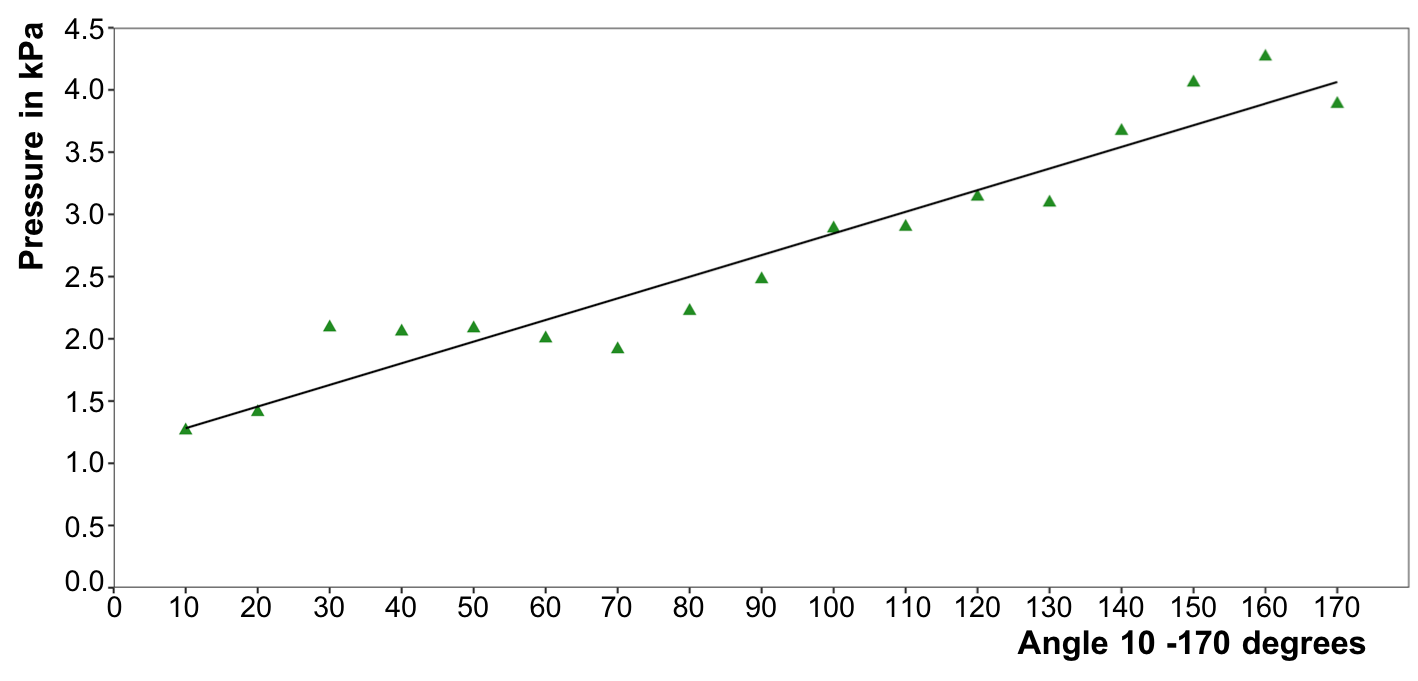
\includegraphics[width=1\linewidth]{figures/a2p}
        \end{tabular}
        \caption{Angle to pressure mapping.}
        \label{fig:angle_to_pressure}
    \end{center}
\end{figure}

As FacePush can make its torque generators rotate to a specific angle, we were interested in how much pressure is provided on the face by FacePush within their rotational range of 0 to 170 degrees. We set up a force sensing resistor to measure the relationship between the pressure exerted against the different rotating angles of the torque generators. Five FlexiForce Pressure Sensors 1 lb\footnote{\url{https://www.tekscan.com/flexiforce-load-force-sensors-and-systems}} were attached to a one-to-one ratio mannequin head. The attached positions were cheekbone (left and right), the upper region of the tail of eyebrow (left and right), and forehead. The torque generators started from their neutral state and rotated through 10 to 170 degrees in steps of 10 degrees each. The motors were driven at their full speed (with a PWM value of 255). Data from the sensor at the forehead were removed since it was discovered that the pressure was primarily distributed on the both sides of the mannequin's face. The values from the remaining four sensors were averaged and a linear equation derived for the mapping between motor angles and the derived pressures as shown in \textcolor{red}{Figure \ref{fig:angle_to_pressure}}: (y = 1.108 + .017x, R$^2 >$ 0.9). The measurement obtained here is the pressure on a single sensor, which is proportional to the total force exerted on the user's face. The total force can be calculated by multiplying the pressure by the contact area of the facial interface of the HMD.

These results confirm the relationship between the angle and the pressure exerted on the face. FacePush can generate either a weak, or a strong, stimulus based on the pressure intensity at different angles. We define two types of stimuli according to their implementation in our example applications. 1) Discrete stimulus: The duration is 0.5 seconds. Thus its impulse increases and decreases instantly; this is utilized in our boxing application. 2) Continuous stimuli: The duration covers the whole application, but the intensity is different among users. In the virtual diving example application, the simulated water current is generated according to the displacement of the player every three frames during rendering VR scene. The stimuli provided by our system allow for a variety of haptic feedback on the face for VR applications. 

